\documentclass[tikz]{minimal}
\usepackage[paperwidth=10cm,paperheight=10cm,margin=0cm]{geometry}
\usepackage{amsmath,bm}
\usepackage{tikz,pgfplots}
\usetikzlibrary{arrows,
	arrows.meta,
	decorations.pathmorphing,
	calc,%
	decorations.pathmorphing,%
	decorations.markings,
	fadings,%
	shadings,%
	positioning,
	spy,
	shapes,
	shapes.geometric,
	shapes.arrows,
	fit,	
	plotmarks,}
	
\usetikzlibrary{pgfplots.colorbrewer}

\begin{document}
\begin{tikzpicture}[remember picture, overlay]
\node[rotate=45,opacity=0.4](sample) at (current page.center){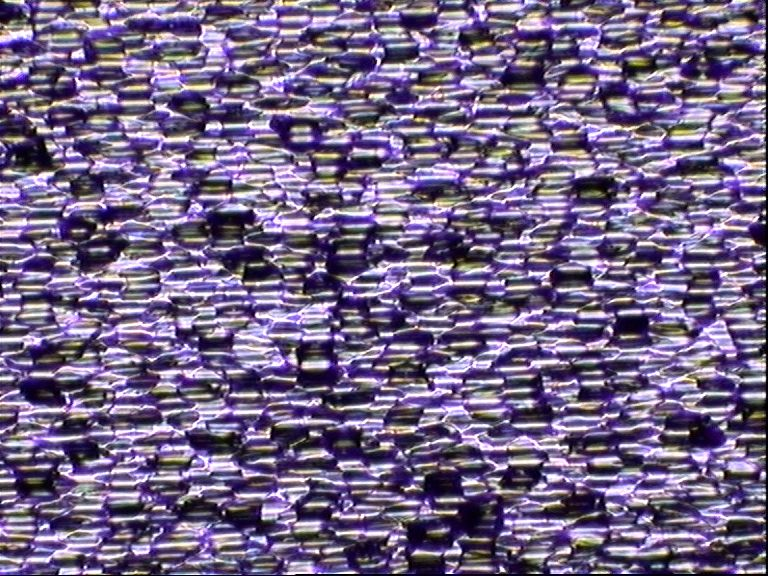
\includegraphics[scale=1]{3522-z2.jpg}};
\draw[-{Stealth[scale=1.5]},shorten >=6.2cm,line width=2mm,color=Set1-B,] (sample.center)--(sample.east);
\draw[-{Stealth[scale=1.5]},shorten >= 3cm,line width=2mm,color=Set1-B,] (sample.center)--(sample.north);
\node[xshift=3cm,yshift=1.5cm,scale=4,color=Set1-B,rotate=45,font=\bfseries] at (sample.center) {$[1\overline{1}0]$};
\node[xshift=-3cm,yshift=1.5cm,scale=4,color=Set1-B,rotate=-45,font=\bfseries] at (sample.center) {$[110]$};
\end{tikzpicture}
\end{document}
	
	